\PassOptionsToPackage{unicode=true}{hyperref} % options for packages loaded elsewhere
\PassOptionsToPackage{hyphens}{url}
%
\documentclass[]{article}
\usepackage{lmodern}
\usepackage{amssymb,amsmath}
\usepackage{ifxetex,ifluatex}
\usepackage{fixltx2e} % provides \textsubscript
\ifnum 0\ifxetex 1\fi\ifluatex 1\fi=0 % if pdftex
  \usepackage[T1]{fontenc}
  \usepackage[utf8]{inputenc}
  \usepackage{textcomp} % provides euro and other symbols
\else % if luatex or xelatex
  \usepackage{unicode-math}
  \defaultfontfeatures{Ligatures=TeX,Scale=MatchLowercase}
\fi
% use upquote if available, for straight quotes in verbatim environments
\IfFileExists{upquote.sty}{\usepackage{upquote}}{}
% use microtype if available
\IfFileExists{microtype.sty}{%
\usepackage[]{microtype}
\UseMicrotypeSet[protrusion]{basicmath} % disable protrusion for tt fonts
}{}
\IfFileExists{parskip.sty}{%
\usepackage{parskip}
}{% else
\setlength{\parindent}{0pt}
\setlength{\parskip}{6pt plus 2pt minus 1pt}
}
\usepackage{hyperref}
\hypersetup{
            pdftitle={Practical 2: Model Evaluation},
            pdfauthor={Laura Rodriguez Navas},
            pdfborder={0 0 0},
            breaklinks=true}
\urlstyle{same}  % don't use monospace font for urls
\usepackage[margin=1in]{geometry}
\usepackage{color}
\usepackage{fancyvrb}
\newcommand{\VerbBar}{|}
\newcommand{\VERB}{\Verb[commandchars=\\\{\}]}
\DefineVerbatimEnvironment{Highlighting}{Verbatim}{commandchars=\\\{\}}
% Add ',fontsize=\small' for more characters per line
\usepackage{framed}
\definecolor{shadecolor}{RGB}{248,248,248}
\newenvironment{Shaded}{\begin{snugshade}}{\end{snugshade}}
\newcommand{\AlertTok}[1]{\textcolor[rgb]{0.94,0.16,0.16}{#1}}
\newcommand{\AnnotationTok}[1]{\textcolor[rgb]{0.56,0.35,0.01}{\textbf{\textit{#1}}}}
\newcommand{\AttributeTok}[1]{\textcolor[rgb]{0.77,0.63,0.00}{#1}}
\newcommand{\BaseNTok}[1]{\textcolor[rgb]{0.00,0.00,0.81}{#1}}
\newcommand{\BuiltInTok}[1]{#1}
\newcommand{\CharTok}[1]{\textcolor[rgb]{0.31,0.60,0.02}{#1}}
\newcommand{\CommentTok}[1]{\textcolor[rgb]{0.56,0.35,0.01}{\textit{#1}}}
\newcommand{\CommentVarTok}[1]{\textcolor[rgb]{0.56,0.35,0.01}{\textbf{\textit{#1}}}}
\newcommand{\ConstantTok}[1]{\textcolor[rgb]{0.00,0.00,0.00}{#1}}
\newcommand{\ControlFlowTok}[1]{\textcolor[rgb]{0.13,0.29,0.53}{\textbf{#1}}}
\newcommand{\DataTypeTok}[1]{\textcolor[rgb]{0.13,0.29,0.53}{#1}}
\newcommand{\DecValTok}[1]{\textcolor[rgb]{0.00,0.00,0.81}{#1}}
\newcommand{\DocumentationTok}[1]{\textcolor[rgb]{0.56,0.35,0.01}{\textbf{\textit{#1}}}}
\newcommand{\ErrorTok}[1]{\textcolor[rgb]{0.64,0.00,0.00}{\textbf{#1}}}
\newcommand{\ExtensionTok}[1]{#1}
\newcommand{\FloatTok}[1]{\textcolor[rgb]{0.00,0.00,0.81}{#1}}
\newcommand{\FunctionTok}[1]{\textcolor[rgb]{0.00,0.00,0.00}{#1}}
\newcommand{\ImportTok}[1]{#1}
\newcommand{\InformationTok}[1]{\textcolor[rgb]{0.56,0.35,0.01}{\textbf{\textit{#1}}}}
\newcommand{\KeywordTok}[1]{\textcolor[rgb]{0.13,0.29,0.53}{\textbf{#1}}}
\newcommand{\NormalTok}[1]{#1}
\newcommand{\OperatorTok}[1]{\textcolor[rgb]{0.81,0.36,0.00}{\textbf{#1}}}
\newcommand{\OtherTok}[1]{\textcolor[rgb]{0.56,0.35,0.01}{#1}}
\newcommand{\PreprocessorTok}[1]{\textcolor[rgb]{0.56,0.35,0.01}{\textit{#1}}}
\newcommand{\RegionMarkerTok}[1]{#1}
\newcommand{\SpecialCharTok}[1]{\textcolor[rgb]{0.00,0.00,0.00}{#1}}
\newcommand{\SpecialStringTok}[1]{\textcolor[rgb]{0.31,0.60,0.02}{#1}}
\newcommand{\StringTok}[1]{\textcolor[rgb]{0.31,0.60,0.02}{#1}}
\newcommand{\VariableTok}[1]{\textcolor[rgb]{0.00,0.00,0.00}{#1}}
\newcommand{\VerbatimStringTok}[1]{\textcolor[rgb]{0.31,0.60,0.02}{#1}}
\newcommand{\WarningTok}[1]{\textcolor[rgb]{0.56,0.35,0.01}{\textbf{\textit{#1}}}}
\usepackage{graphicx,grffile}
\makeatletter
\def\maxwidth{\ifdim\Gin@nat@width>\linewidth\linewidth\else\Gin@nat@width\fi}
\def\maxheight{\ifdim\Gin@nat@height>\textheight\textheight\else\Gin@nat@height\fi}
\makeatother
% Scale images if necessary, so that they will not overflow the page
% margins by default, and it is still possible to overwrite the defaults
% using explicit options in \includegraphics[width, height, ...]{}
\setkeys{Gin}{width=\maxwidth,height=\maxheight,keepaspectratio}
\setlength{\emergencystretch}{3em}  % prevent overfull lines
\providecommand{\tightlist}{%
  \setlength{\itemsep}{0pt}\setlength{\parskip}{0pt}}
\setcounter{secnumdepth}{0}
% Redefines (sub)paragraphs to behave more like sections
\ifx\paragraph\undefined\else
\let\oldparagraph\paragraph
\renewcommand{\paragraph}[1]{\oldparagraph{#1}\mbox{}}
\fi
\ifx\subparagraph\undefined\else
\let\oldsubparagraph\subparagraph
\renewcommand{\subparagraph}[1]{\oldsubparagraph{#1}\mbox{}}
\fi

% set default figure placement to htbp
\makeatletter
\def\fps@figure{htbp}
\makeatother


\title{Practical 2: Model Evaluation}
\author{Laura Rodriguez Navas}
\date{January 2020}

\begin{document}
\maketitle

\hypertarget{section-1}{%
\subsection{Section 1}\label{section-1}}

Load the data into R. Name the columns to better identify the board, as
visited from left to right and from top to down.

\begin{Shaded}
\begin{Highlighting}[]
\NormalTok{data <-}\StringTok{ }\KeywordTok{read.table}\NormalTok{(}\StringTok{"tic-tac-toe.data.txt"}\NormalTok{, }\DataTypeTok{header=}\OtherTok{FALSE}\NormalTok{, }\DataTypeTok{sep=}\StringTok{","}\NormalTok{)}
\KeywordTok{names}\NormalTok{(data) <-}\StringTok{ }\KeywordTok{c}\NormalTok{(}\StringTok{"top-left-square"}\NormalTok{, }
                 \StringTok{"top-middle-square"}\NormalTok{, }
                 \StringTok{"top-right-square"}\NormalTok{, }
                 \StringTok{"middle-left-square"}\NormalTok{, }
                 \StringTok{"middle-middle-square"}\NormalTok{, }
                 \StringTok{"middle-right-square"}\NormalTok{, }
                 \StringTok{"bottom-left-square"}\NormalTok{, }
                 \StringTok{"bottom-middle-square"}\NormalTok{,}
                 \StringTok{"bottom-right-square"}\NormalTok{, }
                 \StringTok{"Class"}\NormalTok{)}
\KeywordTok{str}\NormalTok{(data)}
\end{Highlighting}
\end{Shaded}

\begin{verbatim}
## 'data.frame':    958 obs. of  10 variables:
##  $ top-left-square     : Factor w/ 3 levels "b","o","x": 3 3 3 3 3 3 3 3 3 3 ...
##  $ top-middle-square   : Factor w/ 3 levels "b","o","x": 3 3 3 3 3 3 3 3 3 3 ...
##  $ top-right-square    : Factor w/ 3 levels "b","o","x": 3 3 3 3 3 3 3 3 3 3 ...
##  $ middle-left-square  : Factor w/ 3 levels "b","o","x": 3 3 3 3 3 3 3 3 3 3 ...
##  $ middle-middle-square: Factor w/ 3 levels "b","o","x": 2 2 2 2 2 2 2 2 2 1 ...
##  $ middle-right-square : Factor w/ 3 levels "b","o","x": 2 2 2 2 2 2 1 1 1 2 ...
##  $ bottom-left-square  : Factor w/ 3 levels "b","o","x": 3 2 2 2 1 1 2 2 1 2 ...
##  $ bottom-middle-square: Factor w/ 3 levels "b","o","x": 2 3 2 1 2 1 2 1 2 2 ...
##  $ bottom-right-square : Factor w/ 3 levels "b","o","x": 2 2 3 1 1 2 1 2 2 1 ...
##  $ Class               : Factor w/ 2 levels "negative","positive": 2 2 2 2 2 2 2 2 2 2 ...
\end{verbatim}

Check for missing values.

\begin{Shaded}
\begin{Highlighting}[]
\KeywordTok{any}\NormalTok{(}\KeywordTok{is.na}\NormalTok{(data))}
\end{Highlighting}
\end{Shaded}

\begin{verbatim}
## [1] FALSE
\end{verbatim}

\hypertarget{section-2}{%
\subsection{Section 2}\label{section-2}}

Read the ``data splitting'' section at the web page of caret. Then split
the data into 70\% training and 30\% test by keeping the original
proportion of classes.

\begin{Shaded}
\begin{Highlighting}[]
\KeywordTok{set.seed}\NormalTok{(}\DecValTok{825}\NormalTok{)}
\NormalTok{inTraining <-}\StringTok{ }\KeywordTok{createDataPartition}\NormalTok{(data}\OperatorTok{$}\NormalTok{Class, }\DataTypeTok{p=}\NormalTok{.}\DecValTok{7}\NormalTok{, }\DataTypeTok{list=}\OtherTok{FALSE}\NormalTok{)}
\NormalTok{data_training <-}\StringTok{ }\NormalTok{data[ inTraining,]}
\NormalTok{data_testing  <-}\StringTok{ }\NormalTok{data[}\OperatorTok{-}\NormalTok{inTraining,]}
\KeywordTok{str}\NormalTok{(data_training)}
\end{Highlighting}
\end{Shaded}

\begin{verbatim}
## 'data.frame':    672 obs. of  10 variables:
##  $ top.left.square     : Factor w/ 3 levels "b","o","x": 3 3 3 3 3 3 3 3 3 3 ...
##  $ top.middle.square   : Factor w/ 3 levels "b","o","x": 3 3 3 3 3 3 3 3 3 3 ...
##  $ top.right.square    : Factor w/ 3 levels "b","o","x": 3 3 3 3 3 3 3 3 3 3 ...
##  $ middle.left.square  : Factor w/ 3 levels "b","o","x": 3 3 3 3 3 3 3 3 3 3 ...
##  $ middle.middle.square: Factor w/ 3 levels "b","o","x": 2 2 2 2 2 2 2 2 1 1 ...
##  $ middle.right.square : Factor w/ 3 levels "b","o","x": 2 2 2 2 2 2 1 1 2 2 ...
##  $ bottom.left.square  : Factor w/ 3 levels "b","o","x": 3 2 2 2 1 1 2 2 2 1 ...
##  $ bottom.middle.square: Factor w/ 3 levels "b","o","x": 2 3 2 1 2 1 2 1 2 2 ...
##  $ bottom.right.square : Factor w/ 3 levels "b","o","x": 2 2 3 1 1 2 1 2 1 2 ...
##  $ Class               : Factor w/ 2 levels "negative","positive": 2 2 2 2 2 2 2 2 2 2 ...
\end{verbatim}

\begin{Shaded}
\begin{Highlighting}[]
\KeywordTok{str}\NormalTok{(data_testing)}
\end{Highlighting}
\end{Shaded}

\begin{verbatim}
## 'data.frame':    286 obs. of  10 variables:
##  $ top.left.square     : Factor w/ 3 levels "b","o","x": 3 3 3 3 3 3 3 3 3 3 ...
##  $ top.middle.square   : Factor w/ 3 levels "b","o","x": 3 3 3 3 3 3 3 3 3 3 ...
##  $ top.right.square    : Factor w/ 3 levels "b","o","x": 3 3 3 3 3 3 3 3 3 3 ...
##  $ middle.left.square  : Factor w/ 3 levels "b","o","x": 3 3 2 2 2 2 2 2 2 2 ...
##  $ middle.middle.square: Factor w/ 3 levels "b","o","x": 2 1 3 3 3 3 2 1 1 1 ...
##  $ middle.right.square : Factor w/ 3 levels "b","o","x": 1 2 2 2 2 1 1 3 3 2 ...
##  $ bottom.left.square  : Factor w/ 3 levels "b","o","x": 1 2 3 2 1 2 2 2 1 3 ...
##  $ bottom.middle.square: Factor w/ 3 levels "b","o","x": 2 1 2 1 2 1 1 2 2 2 ...
##  $ bottom.right.square : Factor w/ 3 levels "b","o","x": 2 2 2 1 1 2 3 1 2 1 ...
##  $ Class               : Factor w/ 2 levels "negative","positive": 2 2 2 2 2 2 2 2 2 2 ...
\end{verbatim}

\hypertarget{section-3}{%
\subsection{Section 3}\label{section-3}}

Specifiy the type of resampling.

\begin{Shaded}
\begin{Highlighting}[]
\NormalTok{fitControl <-}\StringTok{ }\KeywordTok{trainControl}\NormalTok{(}\DataTypeTok{method=}\StringTok{"repeatedcv"}\NormalTok{, }
                           \DataTypeTok{number=}\DecValTok{10}\NormalTok{, }
                           \DataTypeTok{repeats=}\DecValTok{1}\NormalTok{,}
                           \DataTypeTok{classProbs=}\OtherTok{TRUE}\NormalTok{)}
\end{Highlighting}
\end{Shaded}

Apply the models: Naive Bayes, Decision Tree, Neural Networks, Nearest
Neighbour and SVM (linear kernel) to the data training dataset using the
same seed.

\begin{enumerate}
\def\labelenumi{\arabic{enumi}.}
\tightlist
\item
  Model Naive Bayes
\end{enumerate}

\begin{Shaded}
\begin{Highlighting}[]
\KeywordTok{set.seed}\NormalTok{(}\DecValTok{825}\NormalTok{)}
\NormalTok{nb <-}\StringTok{ }\KeywordTok{train}\NormalTok{(Class }\OperatorTok{~}\StringTok{ }\NormalTok{., }
            \DataTypeTok{data=}\NormalTok{data_training, }
            \DataTypeTok{method=}\StringTok{"naive_bayes"}\NormalTok{,}
            \DataTypeTok{trControl=}\NormalTok{fitControl)}
\NormalTok{nb}
\end{Highlighting}
\end{Shaded}

\begin{verbatim}
## Naive Bayes 
## 
## 672 samples
##   9 predictor
##   2 classes: 'negative', 'positive' 
## 
## No pre-processing
## Resampling: Cross-Validated (10 fold, repeated 1 times) 
## Summary of sample sizes: 606, 605, 604, 605, 605, 605, ... 
## Resampling results across tuning parameters:
## 
##   usekernel  Accuracy   Kappa    
##   FALSE      0.6756219  0.2666418
##    TRUE      0.6845565  0.1130575
## 
## Tuning parameter 'laplace' was held constant at a value of 0
## Tuning
##  parameter 'adjust' was held constant at a value of 1
## Accuracy was used to select the optimal model using the largest value.
## The final values used for the model were laplace = 0, usekernel = TRUE
##  and adjust = 1.
\end{verbatim}

\begin{enumerate}
\def\labelenumi{\arabic{enumi}.}
\setcounter{enumi}{1}
\tightlist
\item
  Model Decision Tree
\end{enumerate}

\begin{Shaded}
\begin{Highlighting}[]
\KeywordTok{set.seed}\NormalTok{(}\DecValTok{825}\NormalTok{)}
\NormalTok{dt <-}\StringTok{ }\KeywordTok{train}\NormalTok{(Class }\OperatorTok{~}\StringTok{ }\NormalTok{., }
            \DataTypeTok{data=}\NormalTok{data_training, }
            \DataTypeTok{method=}\StringTok{"rpart2"}\NormalTok{,}
            \DataTypeTok{trControl=}\NormalTok{fitControl)}
\NormalTok{dt}
\end{Highlighting}
\end{Shaded}

\begin{verbatim}
## CART 
## 
## 672 samples
##   9 predictor
##   2 classes: 'negative', 'positive' 
## 
## No pre-processing
## Resampling: Cross-Validated (10 fold, repeated 1 times) 
## Summary of sample sizes: 606, 605, 604, 605, 605, 605, ... 
## Resampling results across tuning parameters:
## 
##   maxdepth  Accuracy   Kappa    
##    1        0.6889703  0.3190082
##    5        0.7530403  0.3667066
##   10        0.9107511  0.7973708
## 
## Accuracy was used to select the optimal model using the largest value.
## The final value used for the model was maxdepth = 10.
\end{verbatim}

\begin{enumerate}
\def\labelenumi{\arabic{enumi}.}
\setcounter{enumi}{2}
\tightlist
\item
  Model Neural Network
\end{enumerate}

\begin{Shaded}
\begin{Highlighting}[]
\KeywordTok{set.seed}\NormalTok{(}\DecValTok{825}\NormalTok{)}
\NormalTok{nn <-}\StringTok{ }\KeywordTok{train}\NormalTok{(Class }\OperatorTok{~}\StringTok{ }\NormalTok{., }
            \DataTypeTok{data=}\NormalTok{data_training, }
            \DataTypeTok{method=}\StringTok{"nnet"}\NormalTok{,}
            \DataTypeTok{trControl=}\NormalTok{fitControl)}
\end{Highlighting}
\end{Shaded}

\begin{Shaded}
\begin{Highlighting}[]
\NormalTok{nn}
\end{Highlighting}
\end{Shaded}

\begin{verbatim}
## Neural Network 
## 
## 672 samples
##   9 predictor
##   2 classes: 'negative', 'positive' 
## 
## No pre-processing
## Resampling: Cross-Validated (10 fold, repeated 1 times) 
## Summary of sample sizes: 606, 605, 604, 605, 605, 605, ... 
## Resampling results across tuning parameters:
## 
##   size  decay  Accuracy   Kappa    
##   1     0e+00  0.9732221  0.9402993
##   1     1e-04  0.9717296  0.9369543
##   1     1e-01  0.9776778  0.9498311
##   3     0e+00  0.8646593  0.6307553
##   3     1e-04  0.9612592  0.9140460
##   3     1e-01  0.9776997  0.9499157
##   5     0e+00  0.9598771  0.9103137
##   5     1e-04  0.9582954  0.9085208
##   5     1e-01  0.9761846  0.9466124
## 
## Accuracy was used to select the optimal model using the largest value.
## The final values used for the model were size = 3 and decay = 0.1.
\end{verbatim}

\begin{enumerate}
\def\labelenumi{\arabic{enumi}.}
\setcounter{enumi}{3}
\tightlist
\item
  Model Nearest Neighbour
\end{enumerate}

\begin{Shaded}
\begin{Highlighting}[]
\KeywordTok{set.seed}\NormalTok{(}\DecValTok{825}\NormalTok{)}
\NormalTok{knn <-}\StringTok{ }\KeywordTok{train}\NormalTok{(Class }\OperatorTok{~}\StringTok{ }\NormalTok{., }
             \DataTypeTok{data=}\NormalTok{data_training, }
             \DataTypeTok{method=}\StringTok{"knn"}\NormalTok{,}
             \DataTypeTok{trControl=}\NormalTok{fitControl)}
\NormalTok{knn}
\end{Highlighting}
\end{Shaded}

\begin{verbatim}
## k-Nearest Neighbors 
## 
## 672 samples
##   9 predictor
##   2 classes: 'negative', 'positive' 
## 
## No pre-processing
## Resampling: Cross-Validated (10 fold, repeated 1 times) 
## Summary of sample sizes: 606, 605, 604, 605, 605, 605, ... 
## Resampling results across tuning parameters:
## 
##   k  Accuracy   Kappa    
##   5  0.9420751  0.8667396
##   7  0.8066433  0.5374263
##   9  0.7709534  0.4451248
## 
## Accuracy was used to select the optimal model using the largest value.
## The final value used for the model was k = 5.
\end{verbatim}

\begin{enumerate}
\def\labelenumi{\arabic{enumi}.}
\setcounter{enumi}{4}
\tightlist
\item
  Model SVM (linear kernel)
\end{enumerate}

\begin{Shaded}
\begin{Highlighting}[]
\KeywordTok{set.seed}\NormalTok{(}\DecValTok{825}\NormalTok{)}
\NormalTok{svm <-}\StringTok{ }\KeywordTok{train}\NormalTok{(Class }\OperatorTok{~}\StringTok{ }\NormalTok{., }
             \DataTypeTok{data=}\NormalTok{data_training, }
             \DataTypeTok{method=}\StringTok{"svmLinear"}\NormalTok{,}
             \DataTypeTok{trControl=}\NormalTok{fitControl)}
\NormalTok{svm}
\end{Highlighting}
\end{Shaded}

\begin{verbatim}
## Support Vector Machines with Linear Kernel 
## 
## 672 samples
##   9 predictor
##   2 classes: 'negative', 'positive' 
## 
## No pre-processing
## Resampling: Cross-Validated (10 fold, repeated 1 times) 
## Summary of sample sizes: 606, 605, 604, 605, 605, 605, ... 
## Resampling results:
## 
##   Accuracy   Kappa    
##   0.9806629  0.9563793
## 
## Tuning parameter 'C' was held constant at a value of 1
\end{verbatim}

Collect the results for all the models.

\begin{Shaded}
\begin{Highlighting}[]
\NormalTok{resamps <-}\StringTok{ }\KeywordTok{resamples}\NormalTok{(}\KeywordTok{list}\NormalTok{(}\StringTok{"Naive Bayes"}\NormalTok{=nb,}
                          \StringTok{"Decision Tree"}\NormalTok{=dt,}
                          \StringTok{"Neural Network"}\NormalTok{=nn,}
                          \StringTok{"Nearest Neighbour"}\NormalTok{=knn,}
                          \StringTok{"SVM (linear kernel)"}\NormalTok{=svm))}
\KeywordTok{summary}\NormalTok{(resamps)}
\end{Highlighting}
\end{Shaded}

\begin{verbatim}
## 
## Call:
## summary.resamples(object = resamps)
## 
## Models: Naive Bayes, Decision Tree, Neural Network, Nearest Neighbour, SVM (linear kernel) 
## Number of resamples: 10 
## 
## Accuracy 
##                          Min.   1st Qu.    Median      Mean   3rd Qu.      Max.
## Naive Bayes         0.6567164 0.6642340 0.6865672 0.6845565 0.6943691 0.7205882
## Decision Tree       0.8507463 0.9000668 0.9104478 0.9107511 0.9253731 0.9701493
## Neural Network      0.9552239 0.9702590 0.9850746 0.9776997 0.9852392 1.0000000
## Nearest Neighbour   0.8955224 0.9188982 0.9402985 0.9420751 0.9700362 0.9850746
## SVM (linear kernel) 0.9552239 0.9702590 0.9850746 0.9806629 0.9852392 1.0000000
##                     NA's
## Naive Bayes            0
## Decision Tree          0
## Neural Network         0
## Nearest Neighbour      0
## SVM (linear kernel)    0
## 
## Kappa 
##                          Min.    1st Qu.    Median      Mean   3rd Qu.
## Naive Bayes         0.0000000 0.05403608 0.1111813 0.1130575 0.1504189
## Decision Tree       0.6469968 0.77864355 0.7984862 0.7973708 0.8318554
## Neural Network      0.8975013 0.93288438 0.9665502 0.9499157 0.9672590
## Nearest Neighbour   0.7556019 0.81184946 0.8647830 0.8667396 0.9330473
## SVM (linear kernel) 0.8975013 0.93288438 0.9665502 0.9563793 0.9672590
##                          Max. NA's
## Naive Bayes         0.2540416    0
## Decision Tree       0.9337945    0
## Neural Network      1.0000000    0
## Nearest Neighbour   0.9665502    0
## SVM (linear kernel) 1.0000000    0
\end{verbatim}

Complete the following table with the final values of accuracy and kappa
for the training data:

\begin{center}
	\begin{tabular}{ |c|c|c|c| } 
		\hline
		& Accuracy & Kappa \\
		\hline
		Naive Bayes & 0.6845565 & 0.1130575 \\ 
		Decision Tree & 0.9107511 & 0.7973708 \\ 
		Neural Network & 0.9776997 & 0.9499157 \\
		Nearest Network & 0.9420751 & 0.8667396 \\
		SVM (linear tree) & 0.9806629 & 0.9563793 \\
		\hline
	\end{tabular}
\end{center}

\hypertarget{section-4}{%
\subsection{Section 4}\label{section-4}}

Apply the models: Naive Bayes, Decision Tree, Neural Networks, Nearest
Neighbour and SVM (linear kernel) to the data testing dataset. Print the
confusion matrix of each model.

\begin{enumerate}
\def\labelenumi{\arabic{enumi}.}
\tightlist
\item
  Model Naive Bayes
\end{enumerate}

\begin{Shaded}
\begin{Highlighting}[]
\NormalTok{nbPredict <-}\StringTok{ }\KeywordTok{predict}\NormalTok{(nb, }\DataTypeTok{newdata=}\NormalTok{data_testing)}
\KeywordTok{confusionMatrix}\NormalTok{(nbPredict, data_testing}\OperatorTok{$}\NormalTok{Class)}
\end{Highlighting}
\end{Shaded}

\begin{verbatim}
## Confusion Matrix and Statistics
## 
##           Reference
## Prediction negative positive
##   negative        7        0
##   positive       92      187
##                                           
##                Accuracy : 0.6783          
##                  95% CI : (0.6208, 0.7321)
##     No Information Rate : 0.6538          
##     P-Value [Acc > NIR] : 0.2102          
##                                           
##                   Kappa : 0.0905          
##                                           
##  Mcnemar's Test P-Value : <2e-16          
##                                           
##             Sensitivity : 0.07071         
##             Specificity : 1.00000         
##          Pos Pred Value : 1.00000         
##          Neg Pred Value : 0.67025         
##              Prevalence : 0.34615         
##          Detection Rate : 0.02448         
##    Detection Prevalence : 0.02448         
##       Balanced Accuracy : 0.53535         
##                                           
##        'Positive' Class : negative        
## 
\end{verbatim}

\begin{enumerate}
\def\labelenumi{\arabic{enumi}.}
\setcounter{enumi}{1}
\tightlist
\item
  Model Decision Tree
\end{enumerate}

\begin{Shaded}
\begin{Highlighting}[]
\NormalTok{dtPredict <-}\StringTok{ }\KeywordTok{predict}\NormalTok{(dt, }\DataTypeTok{newdata=}\NormalTok{data_testing)}
\KeywordTok{confusionMatrix}\NormalTok{(dtPredict, data_testing}\OperatorTok{$}\NormalTok{Class)}
\end{Highlighting}
\end{Shaded}

\begin{verbatim}
## Confusion Matrix and Statistics
## 
##           Reference
## Prediction negative positive
##   negative       92       14
##   positive        7      173
##                                          
##                Accuracy : 0.9266         
##                  95% CI : (0.8899, 0.954)
##     No Information Rate : 0.6538         
##     P-Value [Acc > NIR] : <2e-16         
##                                          
##                   Kappa : 0.8404         
##                                          
##  Mcnemar's Test P-Value : 0.1904         
##                                          
##             Sensitivity : 0.9293         
##             Specificity : 0.9251         
##          Pos Pred Value : 0.8679         
##          Neg Pred Value : 0.9611         
##              Prevalence : 0.3462         
##          Detection Rate : 0.3217         
##    Detection Prevalence : 0.3706         
##       Balanced Accuracy : 0.9272         
##                                          
##        'Positive' Class : negative       
## 
\end{verbatim}

\begin{enumerate}
\def\labelenumi{\arabic{enumi}.}
\setcounter{enumi}{2}
\tightlist
\item
  Model Neural Network
\end{enumerate}

\begin{Shaded}
\begin{Highlighting}[]
\NormalTok{nnPredict <-}\StringTok{ }\KeywordTok{predict}\NormalTok{(nn, }\DataTypeTok{newdata=}\NormalTok{data_testing)}
\KeywordTok{confusionMatrix}\NormalTok{(nnPredict, data_testing}\OperatorTok{$}\NormalTok{Class)}
\end{Highlighting}
\end{Shaded}

\begin{verbatim}
## Confusion Matrix and Statistics
## 
##           Reference
## Prediction negative positive
##   negative       96        0
##   positive        3      187
##                                           
##                Accuracy : 0.9895          
##                  95% CI : (0.9697, 0.9978)
##     No Information Rate : 0.6538          
##     P-Value [Acc > NIR] : <2e-16          
##                                           
##                   Kappa : 0.9767          
##                                           
##  Mcnemar's Test P-Value : 0.2482          
##                                           
##             Sensitivity : 0.9697          
##             Specificity : 1.0000          
##          Pos Pred Value : 1.0000          
##          Neg Pred Value : 0.9842          
##              Prevalence : 0.3462          
##          Detection Rate : 0.3357          
##    Detection Prevalence : 0.3357          
##       Balanced Accuracy : 0.9848          
##                                           
##        'Positive' Class : negative        
## 
\end{verbatim}

\begin{enumerate}
\def\labelenumi{\arabic{enumi}.}
\setcounter{enumi}{3}
\tightlist
\item
  Model Nearest Neighbour
\end{enumerate}

\begin{Shaded}
\begin{Highlighting}[]
\NormalTok{knnPredict <-}\StringTok{ }\KeywordTok{predict}\NormalTok{(knn, }\DataTypeTok{newdata=}\NormalTok{data_testing)}
\KeywordTok{confusionMatrix}\NormalTok{(knnPredict, data_testing}\OperatorTok{$}\NormalTok{Class)}
\end{Highlighting}
\end{Shaded}

\begin{verbatim}
## Confusion Matrix and Statistics
## 
##           Reference
## Prediction negative positive
##   negative       92        0
##   positive        7      187
##                                           
##                Accuracy : 0.9755          
##                  95% CI : (0.9502, 0.9901)
##     No Information Rate : 0.6538          
##     P-Value [Acc > NIR] : < 2e-16         
##                                           
##                   Kappa : 0.945           
##                                           
##  Mcnemar's Test P-Value : 0.02334         
##                                           
##             Sensitivity : 0.9293          
##             Specificity : 1.0000          
##          Pos Pred Value : 1.0000          
##          Neg Pred Value : 0.9639          
##              Prevalence : 0.3462          
##          Detection Rate : 0.3217          
##    Detection Prevalence : 0.3217          
##       Balanced Accuracy : 0.9646          
##                                           
##        'Positive' Class : negative        
## 
\end{verbatim}

\begin{enumerate}
\def\labelenumi{\arabic{enumi}.}
\setcounter{enumi}{4}
\tightlist
\item
  Model SVM (linear kernel)
\end{enumerate}

\begin{Shaded}
\begin{Highlighting}[]
\NormalTok{svmPredict <-}\StringTok{ }\KeywordTok{predict}\NormalTok{(svm, }\DataTypeTok{newdata=}\NormalTok{data_testing)}
\KeywordTok{confusionMatrix}\NormalTok{(svmPredict, data_testing}\OperatorTok{$}\NormalTok{Class)}
\end{Highlighting}
\end{Shaded}

\begin{verbatim}
## Confusion Matrix and Statistics
## 
##           Reference
## Prediction negative positive
##   negative       96        0
##   positive        3      187
##                                           
##                Accuracy : 0.9895          
##                  95% CI : (0.9697, 0.9978)
##     No Information Rate : 0.6538          
##     P-Value [Acc > NIR] : <2e-16          
##                                           
##                   Kappa : 0.9767          
##                                           
##  Mcnemar's Test P-Value : 0.2482          
##                                           
##             Sensitivity : 0.9697          
##             Specificity : 1.0000          
##          Pos Pred Value : 1.0000          
##          Neg Pred Value : 0.9842          
##              Prevalence : 0.3462          
##          Detection Rate : 0.3357          
##    Detection Prevalence : 0.3357          
##       Balanced Accuracy : 0.9848          
##                                           
##        'Positive' Class : negative        
## 
\end{verbatim}

Calculate the AUC value for all the models.

\begin{enumerate}
\def\labelenumi{\arabic{enumi}.}
\tightlist
\item
  Model Naive Bayes
\end{enumerate}

\begin{Shaded}
\begin{Highlighting}[]
\KeywordTok{auc}\NormalTok{(}\KeywordTok{roc}\NormalTok{(nbPredict, data_testing}\OperatorTok{$}\NormalTok{Class))}
\end{Highlighting}
\end{Shaded}

\begin{verbatim}
## [1] 0.5353535
\end{verbatim}

\begin{enumerate}
\def\labelenumi{\arabic{enumi}.}
\setcounter{enumi}{1}
\tightlist
\item
  Model Decison Tree
\end{enumerate}

\begin{Shaded}
\begin{Highlighting}[]
\KeywordTok{auc}\NormalTok{(}\KeywordTok{roc}\NormalTok{(dtPredict, data_testing}\OperatorTok{$}\NormalTok{Class))}
\end{Highlighting}
\end{Shaded}

\begin{verbatim}
## [1] 0.9272133
\end{verbatim}

\begin{enumerate}
\def\labelenumi{\arabic{enumi}.}
\setcounter{enumi}{2}
\tightlist
\item
  Model Neural Network
\end{enumerate}

\begin{Shaded}
\begin{Highlighting}[]
\KeywordTok{auc}\NormalTok{(}\KeywordTok{roc}\NormalTok{(nnPredict, data_testing}\OperatorTok{$}\NormalTok{Class))}
\end{Highlighting}
\end{Shaded}

\begin{verbatim}
## [1] 0.9848485
\end{verbatim}

\begin{enumerate}
\def\labelenumi{\arabic{enumi}.}
\setcounter{enumi}{3}
\tightlist
\item
  Model Nearest Network
\end{enumerate}

\begin{Shaded}
\begin{Highlighting}[]
\KeywordTok{auc}\NormalTok{(}\KeywordTok{roc}\NormalTok{(knnPredict, data_testing}\OperatorTok{$}\NormalTok{Class))}
\end{Highlighting}
\end{Shaded}

\begin{verbatim}
## [1] 0.9646465
\end{verbatim}

\begin{enumerate}
\def\labelenumi{\arabic{enumi}.}
\setcounter{enumi}{4}
\tightlist
\item
  Model SVM (linear kernel)
\end{enumerate}

\begin{Shaded}
\begin{Highlighting}[]
\KeywordTok{auc}\NormalTok{(}\KeywordTok{roc}\NormalTok{(svmPredict, data_testing}\OperatorTok{$}\NormalTok{Class))}
\end{Highlighting}
\end{Shaded}

\begin{verbatim}
## [1] 0.9848485
\end{verbatim}

Complete the following table with the final values of accuracy, kappa
and AUC for the testing data.

\begin{center}
	\begin{tabular}{ |c|c|c|c| } 
		\hline
		& Accuracy & Kappa & AUC \\
		\hline
		Naive Bayes & 0.6783 & 0.0905 & 0.5353535 \\ 
		Decision Tree & 0.9266 & 0.8404 & 0.9272133 \\ 
		Neural Network & 0.9895 & 0.9767 & 0.9848485 \\ 
		Nearest Network & 0.9755 & 0.945 & 0.9646465 \\ 
		SVM (linear tree) & 0.9895 & 0.9767 & 0.9848485 \\ 
		\hline
	\end{tabular}
\end{center}

\hypertarget{section-5}{%
\subsection{Section 5}\label{section-5}}

Plot the ROC curves of the models.

\begin{enumerate}
\def\labelenumi{\alph{enumi})}
\tightlist
\item
  Calculate again the predictions on the test set but now setting the
  type parameter of the predict function to ``prob''.
\end{enumerate}

\begin{enumerate}
\def\labelenumi{\arabic{enumi}.}
\tightlist
\item
  Model Naive Bayes
\end{enumerate}

\begin{Shaded}
\begin{Highlighting}[]
\NormalTok{nbPredictProb <-}\StringTok{ }\KeywordTok{predict}\NormalTok{(nb, }\DataTypeTok{newdata=}\NormalTok{data_testing, }\DataTypeTok{type =} \StringTok{"prob"}\NormalTok{)}
\KeywordTok{head}\NormalTok{(nbPredictProb)}
\end{Highlighting}
\end{Shaded}

\begin{verbatim}
##      negative  positive
## 1 0.105410725 0.8945893
## 2 0.048803363 0.9511966
## 3 0.002235508 0.9977645
## 4 0.004361079 0.9956389
## 5 0.001757359 0.9982426
## 6 0.012029302 0.9879707
\end{verbatim}

\begin{enumerate}
\def\labelenumi{\arabic{enumi}.}
\setcounter{enumi}{1}
\tightlist
\item
  Model Decision Tree
\end{enumerate}

\begin{Shaded}
\begin{Highlighting}[]
\NormalTok{dtPredictProb <-}\StringTok{ }\KeywordTok{predict}\NormalTok{(dt, }\DataTypeTok{newdata=}\NormalTok{data_testing, }\DataTypeTok{type =} \StringTok{"prob"}\NormalTok{)}
\KeywordTok{head}\NormalTok{(dtPredictProb)}
\end{Highlighting}
\end{Shaded}

\begin{verbatim}
##    negative positive
## 9      0.00     1.00
## 11     0.16     0.84
## 13     0.00     1.00
## 16     0.00     1.00
## 17     0.00     1.00
## 20     0.16     0.84
\end{verbatim}

\begin{enumerate}
\def\labelenumi{\arabic{enumi}.}
\setcounter{enumi}{2}
\tightlist
\item
  Model Neural Network
\end{enumerate}

\begin{Shaded}
\begin{Highlighting}[]
\NormalTok{nnPredictProb <-}\StringTok{ }\KeywordTok{predict}\NormalTok{(nn, }\DataTypeTok{newdata=}\NormalTok{data_testing, }\DataTypeTok{type =} \StringTok{"prob"}\NormalTok{)}
\KeywordTok{head}\NormalTok{(nnPredictProb)}
\end{Highlighting}
\end{Shaded}

\begin{verbatim}
##       negative  positive
## 9  0.014915208 0.9850848
## 11 0.022068633 0.9779314
## 13 0.018293877 0.9817061
## 16 0.009860493 0.9901395
## 17 0.005332153 0.9946678
## 20 0.015123710 0.9848763
\end{verbatim}

\begin{enumerate}
\def\labelenumi{\arabic{enumi}.}
\setcounter{enumi}{3}
\tightlist
\item
  Model Nearest Neighbour
\end{enumerate}

\begin{Shaded}
\begin{Highlighting}[]
\NormalTok{knnPredictProb <-}\StringTok{ }\KeywordTok{predict}\NormalTok{(knn, }\DataTypeTok{newdata=}\NormalTok{data_testing, }\DataTypeTok{type =} \StringTok{"prob"}\NormalTok{)}
\KeywordTok{head}\NormalTok{(knnPredictProb)}
\end{Highlighting}
\end{Shaded}

\begin{verbatim}
##   negative positive
## 1        0        1
## 2        0        1
## 3        0        1
## 4        0        1
## 5        0        1
## 6        0        1
\end{verbatim}

\begin{enumerate}
\def\labelenumi{\arabic{enumi}.}
\setcounter{enumi}{4}
\tightlist
\item
  Model SVM (linear kernel)
\end{enumerate}

\begin{Shaded}
\begin{Highlighting}[]
\NormalTok{svmPredictProb <-}\StringTok{ }\KeywordTok{predict}\NormalTok{(svm, }\DataTypeTok{newdata=}\NormalTok{data_testing, }\DataTypeTok{type =} \StringTok{"prob"}\NormalTok{)}
\KeywordTok{head}\NormalTok{(svmPredictProb)}
\end{Highlighting}
\end{Shaded}

\begin{verbatim}
##     negative  positive
## 1 0.03087548 0.9691245
## 2 0.03086058 0.9691394
## 3 0.03082860 0.9691714
## 4 0.03084267 0.9691573
## 5 0.03084003 0.9691600
## 6 0.03085089 0.9691491
\end{verbatim}

\begin{enumerate}
\def\labelenumi{\alph{enumi})}
\setcounter{enumi}{1}
\tightlist
\item
  Construct a ``prediction'' object for each classifier using the vector
  of estimated probabilities for the positive class as the first
  parameter, and the vector of actual class labels as the second
  parameter.
\end{enumerate}

\begin{enumerate}
\def\labelenumi{\arabic{enumi}.}
\tightlist
\item
  Model Naive Bayes
\end{enumerate}

\begin{Shaded}
\begin{Highlighting}[]
\NormalTok{nbPred <-}\StringTok{ }\KeywordTok{prediction}\NormalTok{(nbPredictProb}\OperatorTok{$}\NormalTok{positive, data_testing}\OperatorTok{$}\NormalTok{Class)   }
\end{Highlighting}
\end{Shaded}

\begin{enumerate}
\def\labelenumi{\arabic{enumi}.}
\setcounter{enumi}{1}
\tightlist
\item
  Model Decision Tree
\end{enumerate}

\begin{Shaded}
\begin{Highlighting}[]
\NormalTok{dtPred <-}\StringTok{ }\KeywordTok{prediction}\NormalTok{(dtPredictProb}\OperatorTok{$}\NormalTok{positive, data_testing}\OperatorTok{$}\NormalTok{Class)   }
\end{Highlighting}
\end{Shaded}

\begin{enumerate}
\def\labelenumi{\arabic{enumi}.}
\setcounter{enumi}{2}
\tightlist
\item
  Model Neural Network
\end{enumerate}

\begin{Shaded}
\begin{Highlighting}[]
\NormalTok{nnPred <-}\StringTok{ }\KeywordTok{prediction}\NormalTok{(nnPredictProb}\OperatorTok{$}\NormalTok{positive, data_testing}\OperatorTok{$}\NormalTok{Class)   }
\end{Highlighting}
\end{Shaded}

\begin{enumerate}
\def\labelenumi{\arabic{enumi}.}
\setcounter{enumi}{3}
\tightlist
\item
  Model Nearest Neighbour
\end{enumerate}

\begin{Shaded}
\begin{Highlighting}[]
\NormalTok{knnPred <-}\StringTok{ }\KeywordTok{prediction}\NormalTok{(knnPredictProb}\OperatorTok{$}\NormalTok{positive, data_testing}\OperatorTok{$}\NormalTok{Class)   }
\end{Highlighting}
\end{Shaded}

\begin{enumerate}
\def\labelenumi{\arabic{enumi}.}
\setcounter{enumi}{4}
\tightlist
\item
  Model SVM (linear kernel)
\end{enumerate}

\begin{Shaded}
\begin{Highlighting}[]
\NormalTok{svmPred <-}\StringTok{ }\KeywordTok{prediction}\NormalTok{(svmPredictProb}\OperatorTok{$}\NormalTok{positive, data_testing}\OperatorTok{$}\NormalTok{Class)   }
\end{Highlighting}
\end{Shaded}

\begin{enumerate}
\def\labelenumi{\alph{enumi})}
\setcounter{enumi}{2}
\tightlist
\item
  Calculate the measures we want to plot on the y-axis (TPR) and on the
  x-axis (FPR) by using the performance function.
\end{enumerate}

\begin{enumerate}
\def\labelenumi{\arabic{enumi}.}
\tightlist
\item
  Model Naive Bayes
\end{enumerate}

\begin{Shaded}
\begin{Highlighting}[]
\NormalTok{nbPerf <-}\StringTok{ }\KeywordTok{performance}\NormalTok{(nbPred, }\StringTok{"tpr"}\NormalTok{, }\StringTok{"fpr"}\NormalTok{)}
\end{Highlighting}
\end{Shaded}

\begin{enumerate}
\def\labelenumi{\arabic{enumi}.}
\setcounter{enumi}{1}
\tightlist
\item
  Model Decision Tree
\end{enumerate}

\begin{Shaded}
\begin{Highlighting}[]
\NormalTok{dtPerf <-}\StringTok{ }\KeywordTok{performance}\NormalTok{(dtPred, }\StringTok{"tpr"}\NormalTok{, }\StringTok{"fpr"}\NormalTok{)}
\end{Highlighting}
\end{Shaded}

\begin{enumerate}
\def\labelenumi{\arabic{enumi}.}
\setcounter{enumi}{2}
\tightlist
\item
  Model Neural Network
\end{enumerate}

\begin{Shaded}
\begin{Highlighting}[]
\NormalTok{nnPerf <-}\StringTok{ }\KeywordTok{performance}\NormalTok{(nnPred, }\StringTok{"tpr"}\NormalTok{, }\StringTok{"fpr"}\NormalTok{)}
\end{Highlighting}
\end{Shaded}

\begin{enumerate}
\def\labelenumi{\arabic{enumi}.}
\setcounter{enumi}{3}
\tightlist
\item
  Model Nearest Neighbour
\end{enumerate}

\begin{Shaded}
\begin{Highlighting}[]
\NormalTok{knnPerf <-}\StringTok{ }\KeywordTok{performance}\NormalTok{(knnPred, }\StringTok{"tpr"}\NormalTok{, }\StringTok{"fpr"}\NormalTok{)}
\end{Highlighting}
\end{Shaded}

\begin{enumerate}
\def\labelenumi{\arabic{enumi}.}
\setcounter{enumi}{4}
\tightlist
\item
  Model SVM (linear kernel)
\end{enumerate}

\begin{Shaded}
\begin{Highlighting}[]
\NormalTok{svmPerf <-}\StringTok{ }\KeywordTok{performance}\NormalTok{(svmPred, }\StringTok{"tpr"}\NormalTok{, }\StringTok{"fpr"}\NormalTok{)}
\end{Highlighting}
\end{Shaded}

\begin{enumerate}
\def\labelenumi{\alph{enumi})}
\setcounter{enumi}{3}
\tightlist
\item
  Draw all the curves in the same plot.
\end{enumerate}

\begin{Shaded}
\begin{Highlighting}[]
\KeywordTok{plot}\NormalTok{(nbPerf, }\DataTypeTok{col=}\StringTok{"orange"}\NormalTok{, }\DataTypeTok{add=}\OtherTok{FALSE}\NormalTok{, }\DataTypeTok{main=}\StringTok{"Curvas ROC"}\NormalTok{)}
\KeywordTok{plot}\NormalTok{(dtPerf, }\DataTypeTok{col=}\StringTok{"blue"}\NormalTok{, }\DataTypeTok{add=}\OtherTok{TRUE}\NormalTok{, }\DataTypeTok{main=}\StringTok{"Curvas ROC"}\NormalTok{)}
\KeywordTok{plot}\NormalTok{(nnPerf, }\DataTypeTok{col=}\StringTok{"red"}\NormalTok{, }\DataTypeTok{add=}\OtherTok{TRUE}\NormalTok{, }\DataTypeTok{main=}\StringTok{"Curvas ROC"}\NormalTok{)}
\KeywordTok{plot}\NormalTok{(knnPerf, }\DataTypeTok{col=}\StringTok{"green"}\NormalTok{, }\DataTypeTok{add=}\OtherTok{TRUE}\NormalTok{, }\DataTypeTok{main=}\StringTok{"Curvas ROC"}\NormalTok{)}
\KeywordTok{plot}\NormalTok{(svmPerf, }\DataTypeTok{col=}\StringTok{"magenta"}\NormalTok{, }\DataTypeTok{add=}\OtherTok{TRUE}\NormalTok{, }\DataTypeTok{main=}\StringTok{"Curvas ROC"}\NormalTok{)}
\KeywordTok{legend}\NormalTok{(}\StringTok{"bottomright"}\NormalTok{, }
       \DataTypeTok{legend =} \KeywordTok{c}\NormalTok{(}\StringTok{"NB"}\NormalTok{,}\StringTok{"DT"}\NormalTok{, }\StringTok{"NN"}\NormalTok{, }\StringTok{"kNN"}\NormalTok{, }\StringTok{"SVM"}\NormalTok{), }
       \DataTypeTok{col =} \KeywordTok{c}\NormalTok{(}\StringTok{"orange"}\NormalTok{, }\StringTok{"blue"}\NormalTok{, }\StringTok{"red"}\NormalTok{, }\StringTok{"green"}\NormalTok{, }\StringTok{"magenta"}\NormalTok{), }
       \DataTypeTok{lty =} \DecValTok{1}\NormalTok{, }\DataTypeTok{lwd =} \DecValTok{1}\NormalTok{)}
\end{Highlighting}
\end{Shaded}

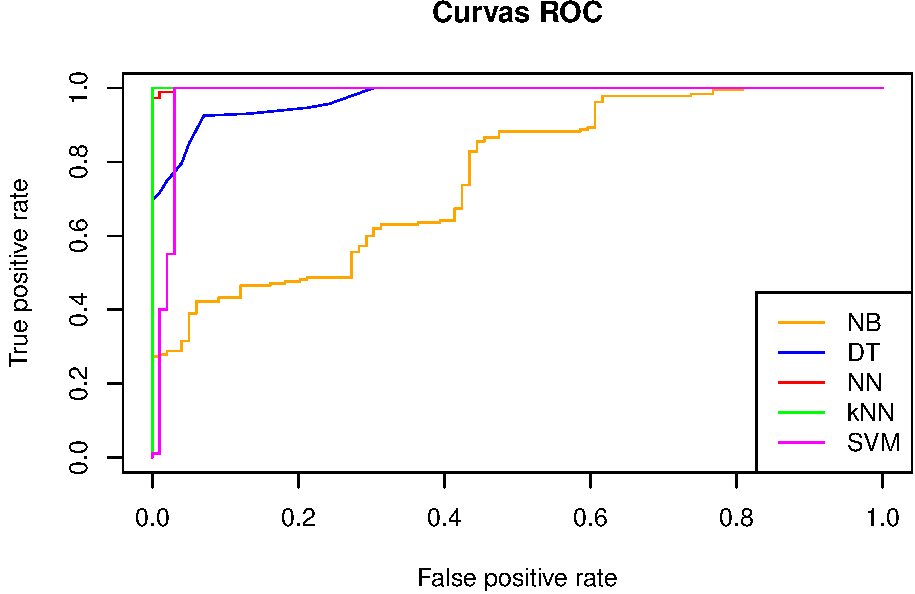
\includegraphics{document_files/figure-latex/unnamed-chunk-44-1.pdf}

\hypertarget{question-1}{%
	\subsection{Question 1. ¿Si el modelo A tiene mayor Accuracy que B, siempre tendrá mayor Kappa que B? Justifica tu respuesta.}\label{question-1}}

Sí, porqué los valores Accuracy y Kappa están relacionados, ya que son considerados dos medidas de exactitud en la técnica de validación cruzada utilizada durante esta práctica. Concretamente, el valor Accuracy representa la exactitud en el porcentaje de aciertos del modelo clasificador, y el valor Kappa representa la concordancia de este, es decir, una medida que valora y valida la exactitud lograda en cada clasificación realizada por el modelo clasificador. Así que, si un modelo clasificador A, tiene mayor Accuracy que un modelo clasificador B, también tendrá mayor Kappa, porqué un modelo con poca coincidencia de aciertos, no puede obtener un alto porcentaje de aciertos. Estas medidas están relacionadas y un alto porcentaje de aciertos implicará una alta coincidencia.

\hypertarget{question-2}{%
	\subsection{Question 2. ¿Vemos eso en tus resultados?}\label{question-2}}

Sí. Si nos fijamos en la primera tabla de resultados de la \ref{section-3}{section 3} podemos observar que el modelo SVM (linear kernel) tiene el valor más alto de Accuracy y siempre tiene mayor Kappa que el resto de modelos. Lo mismo sucede si seguimos comparando, por ejemplo con el modelo Nearest Neighbour con el resto de modelos. El valor Accuracy es mayor y el valor Kappa también. Contrariamente, como el valor Accuracy y Kappa del modelo Nearest Neighbour es menor que en el modelo SVM (linear kernel), no se cumple la pregunta formulada anteriormente.

\hypertarget{question-3}{%
	\subsection{Question 3. ¿Te cambian los resultados cuando cambias la semilla?}\label{question-3}}

Sí. Como se puede observar en las secciones anteriores la semilla utilizada es 825 y la tabla resultante recordamos que ha sido:

\begin{center}
	\begin{tabular}{ |c|c|c|c| } 
		\hline
		& Accuracy & Kappa \\
		\hline
		Naive Bayes & 0.6845565 & 0.1130575 \\ 
		Decision Tree & 0.9107511 & 0.7973708 \\ 
		Neural Network & 0.9776997 & 0.9499157 \\
		Nearest Network & 0.9420751 & 0.8667396 \\
		SVM (linear tree) & 0.9806629 & 0.9563793 \\
		\hline
	\end{tabular}
\end{center}

Aplicando una semilla diferente, por ejemplo utilizando la semilla 123, el resultado es diferente como podemos ver a continuación:

\begin{enumerate}
	\def\labelenumi{\arabic{enumi}.}
	\tightlist
	\item
	Model Naive Bayes
\end{enumerate}

\begin{Shaded}
	\begin{Highlighting}[]
\KeywordTok{set.seed}\NormalTok{(}\DecValTok{123}\NormalTok{)}
\NormalTok{nb <-}\StringTok{ }\KeywordTok{train}\NormalTok{(Class }\OperatorTok{~}\StringTok{ }\NormalTok{., }
	\DataTypeTok{data=}\NormalTok{data_training, }
	\DataTypeTok{method=}\StringTok{"naive_bayes"}\NormalTok{,}
	\DataTypeTok{trControl=}\NormalTok{fitControl)}
	\end{Highlighting}
\end{Shaded}

\begin{enumerate}
	\def\labelenumi{\arabic{enumi}.}
	\setcounter{enumi}{1}
	\tightlist
	\item
	Model Decision Tree
\end{enumerate}

\begin{Shaded}
	\begin{Highlighting}[]
\KeywordTok{set.seed}\NormalTok{(}\DecValTok{123}\NormalTok{)}
\NormalTok{dt <-}\StringTok{ }\KeywordTok{train}\NormalTok{(Class }\OperatorTok{~}\StringTok{ }\NormalTok{., }
	\DataTypeTok{data=}\NormalTok{data_training, }
	\DataTypeTok{method=}\StringTok{"rpart2"}\NormalTok{,}
	\DataTypeTok{trControl=}\NormalTok{fitControl)}
	\end{Highlighting}
\end{Shaded}

\begin{enumerate}
	\def\labelenumi{\arabic{enumi}.}
	\setcounter{enumi}{2}
	\tightlist
	\item
	Model Neural Network
\end{enumerate}

\begin{Shaded}
	\begin{Highlighting}[]
\KeywordTok{set.seed}\NormalTok{(}\DecValTok{123}\NormalTok{)}
\NormalTok{nn <-}\StringTok{ }\KeywordTok{train}\NormalTok{(Class }\OperatorTok{~}\StringTok{ }\NormalTok{., }
	\DataTypeTok{data=}\NormalTok{data_training, }
	\DataTypeTok{method=}\StringTok{"nnet"}\NormalTok{,}
	\DataTypeTok{trControl=}\NormalTok{fitControl)}
	\end{Highlighting}
\end{Shaded}

\begin{enumerate}
	\def\labelenumi{\arabic{enumi}.}
	\setcounter{enumi}{3}
	\tightlist
	\item
	Model Nearest Neighbour
\end{enumerate}

\begin{Shaded}
	\begin{Highlighting}[]
\KeywordTok{set.seed}\NormalTok{(}\DecValTok{123}\NormalTok{)}
\NormalTok{knn <-}\StringTok{ }\KeywordTok{train}\NormalTok{(Class }\OperatorTok{~}\StringTok{ }\NormalTok{., }
	\DataTypeTok{data=}\NormalTok{data_training, }
	\DataTypeTok{method=}\StringTok{"knn"}\NormalTok{,}
	\DataTypeTok{trControl=}\NormalTok{fitControl)}
	\end{Highlighting}
\end{Shaded}

\begin{enumerate}
	\def\labelenumi{\arabic{enumi}.}
	\setcounter{enumi}{4}
	\tightlist
	\item
	Model SVM (linear kernel)
\end{enumerate}

\begin{Shaded}
	\begin{Highlighting}[]
\KeywordTok{set.seed}\NormalTok{(}\DecValTok{123}\NormalTok{)}
\NormalTok{svm <-}\StringTok{ }\KeywordTok{train}\NormalTok{(Class }\OperatorTok{~}\StringTok{ }\NormalTok{., }
	\DataTypeTok{data=}\NormalTok{data_training, }
	\DataTypeTok{method=}\StringTok{"svmLinear"}\NormalTok{,}
	\DataTypeTok{trControl=}\NormalTok{fitControl)}
	\end{Highlighting}
\end{Shaded}

\begin{Shaded}
	\begin{Highlighting}[]
\NormalTok{resamps <-}\StringTok{ }\KeywordTok{resamples}\NormalTok{(}\KeywordTok{list}\NormalTok{(}\StringTok{"Naive Bayes"}\NormalTok{=nb,}
			\StringTok{"Decision Tree"}\NormalTok{=dt,}
			\StringTok{"Neural Network"}\NormalTok{=nn,}
			\StringTok{"Nearest Neighbour"}\NormalTok{=knn,}
			\StringTok{"SVM (linear kernel)"}\NormalTok{=svm))}
\KeywordTok{summary}\NormalTok{(resamps)}
	\end{Highlighting}
\end{Shaded}

\begin{verbatim}
## 
## Call:
## summary.resamples(object = resamps)
## 
## Models: Naive Bayes, Decision Tree, Neural Network, Nearest Neighbour, SVM (linear kernel) 
## Number of resamples: 10 
## 
## Accuracy 
##                          Min.   1st Qu.    Median      Mean   3rd Qu.      Max.
## Naive Bayes         0.6417910 0.6716418 0.6940299 0.7021291 0.7126866 0.7941176
## Decision Tree       0.8235294 0.8544776 0.8964004 0.8974539 0.9253731 0.9701493
## Neural Network      0.9701493 0.9702590 0.9850746 0.9791703 0.9850746 0.9852941
## Nearest Neighbour   0.8805970 0.9107770 0.9402985 0.9360184 0.9665825 0.9701493
## SVM (linear kernel) 0.9701493 0.9702590 0.9850746 0.9806629 0.9850746 1.0000000
##                     NA's
## Naive Bayes            0
## Decision Tree          0
## Neural Network         0
## Nearest Neighbour      0
## SVM (linear kernel)    0
## 
## Kappa 
##                          Min.   1st Qu.    Median      Mean   3rd Qu.      Max.
## Naive Bayes         0.1886983 0.2728508 0.2973763 0.3301961 0.3446200 0.5576208
## Decision Tree       0.5732218 0.6782198 0.7673132 0.7653352 0.8318554 0.9350775
## Neural Network      0.9323915 0.9328844 0.9665502 0.9533158 0.9670654 0.9674952
## Nearest Neighbour   0.7112069 0.7982758 0.8644097 0.8534526 0.9244398 0.9337945
## SVM (linear kernel) 0.9323915 0.9328844 0.9665502 0.9565920 0.9670654 1.0000000
##                     NA's
## Naive Bayes            0
## Decision Tree          0
## Neural Network         0
## Nearest Neighbour      0
## SVM (linear kernel)    0
\end{verbatim}

\hypertarget{question-4}{%
	\subsection{Question 4. ¿Es recomendable quedarse con los resultados mejores después de cambiar las semillas varias veces? Justifica la respuesta.}\label{question-4}}

No. Porqué en estos casos la calibración es aleatoria y no podemos valorar cuales son los mejores resultados entre ellos. Además, con una probabilidad de entrenamiento del 70\%, la calibración se considera perfecta y el primer resultado ya se podría considerar como el mejor.

\hypertarget{question-5}{%
	\subsection{Question 5. ¿Qué modelos puedes descartar porque van a ser siempre menos óptimos (asumiendo una buena evaluación)?}\label{question-5}}

Los modelos Naive Bayes y Decision Tree.

\hypertarget{question-6}{%
	\subsection{Question 6.  ¿Por qué puedes descartar esos modelos?}\label{question-6}}

Si nos fijamos en el gráfico de Curvas ROC que representa el análisis ROC que hemos realizado en esta práctica, podemos descartar estos modelos porqué están por debajo del casco convexo formado por todos los clasificadores considerados, y además no constan en ninguna de las buenas zonas o zonas de dominancia.

\end{document}
